% ============================================================================
%  C2 Alert Tracking and Monitor -- Deliverable #2 component design
%  Owner: Prathamesh Ravindra Sawant
% ============================================================================

\section{Component Overview}

\subsection{Purpose}
C2 Alert Tracking and Monitor is the component that turns a detection into an alert and carries that
alert through its life. It defines alert rules per house, evaluates each detection C3 produces
against the house's enabled rules and service settings, raises an alert on a match, notifies the
house's emergency contacts by email through Amazon SNS, and tracks the alert through its status
machine. It also serves a read-only view of one alert to an external recipient through a signed,
time-limited link, with no login.

C2 owns steps 5, 6 and 7 of the clip-to-alert flow. C3 calls \texttt{POST /alerts/evaluate} after it
stores a detection; C2 decides whether to raise an alert and, if so, notifies contacts. C2 performs
no classification and ingests no clips.

\subsection{Objectives}
\begin{enumerate}
\item Let cloud staff define and tune alert rules per house or per tenant: alert type, severity, trigger labels,
minimum confidence and room.
\item Evaluate each detection deterministically and raise an \texttt{open} alert only when a rule
matches and the service is enabled. The same detection never creates two alerts (idempotent evaluation).
\item Notify emergency contacts in priority order by email, each email carrying a signed link that
expires 24 hours after the alert is triggered. Retry failed emails up to three times.
\item Enforce the alert status machine so an alert can move only along the allowed transitions, and
reject anything else with \texttt{409 invalid\_state}.
\item Record every status change with the actor, role, time and note, for audit.
\item Give the C4 dashboards a query and reporting API: filtered alert lists, alert detail and alert counts.
\end{enumerate}

\subsection{Function scope}
\begin{longtable}{L{6.4cm}L{8.4cm}}
\caption{C2 function scope}\label{tab:c2-scope}\\
\toprule
\textbf{In C2} & \textbf{Out of C2 (owner)} \\
\midrule
\endfirsthead
\caption[]{C2 function scope (continued)}\\
\toprule
\textbf{In C2} & \textbf{Out of C2 (owner)} \\
\midrule
\endhead
Alert types, alert rules, rule evaluation & Clip classification and detections (C3) \\
Alert creation, the status machine, status history & Clip ingestion and feeds (C1) \\
Emergency-contact email via Amazon SNS, notification records and retries & Contact records and house service settings (C4, read-only to C2) \\
Signed, time-limited alert view for external recipients & Authentication, user accounts, JWT issuing (C4) \\
Alert query and reporting APIs & The dashboards that display alerts (C4) \\
\bottomrule
\end{longtable}

\textbf{Assumptions and constraints.} (1) C4 issues the user JWT and C2 only validates it. (2) The
home-label vocabulary is the seven-label C3 label map (TBD-1, resolved by C3). (3) C2 reads C3 and C4
data through read-only gateways and never writes another component's data. (4) Measured latency and
scaling thresholds stay open for Deliverable~\#3 (TBD-3, TBD-5).

\subsection{Usage}
Cloud staff manage rules in the Alert Rules page. House owners act on alerts through Alert Detail:
acknowledge, resolve or mark a false positive. The C3 inference worker is a system caller that
triggers evaluation. External recipients, who hold no account, open the signed alert view from the
link in their email. Table~\ref{tab:c2-actors} summarises who uses C2 and through which interface.

\begin{longtable}{L{3.2cm}L{3.6cm}L{8.0cm}}
\caption{C2 actors and their use of the component}\label{tab:c2-actors}\\
\toprule
\textbf{Actor} & \textbf{Interface} & \textbf{Typical use} \\
\midrule
\endfirsthead
\caption[]{C2 actors and their use of the component (continued)}\\
\toprule
\textbf{Actor} & \textbf{Interface} & \textbf{Typical use} \\
\midrule
\endhead
\texttt{house\_owner} & C4 owner dashboard $\rightarrow$ C2 REST & View alerts of own houses; acknowledge, resolve, mark false positive \\
\texttt{cloud\_staff} & C4 cloud dashboard $\rightarrow$ C2 REST & Manage alert rules for the tenant; view and act on any alert in the tenant; reports \\
C3 inference worker & Internal REST, service JWT & Submit each stored detection for evaluation \\
Emergency contact & Email link $\rightarrow$ public REST & Open the read-only signed alert view (no account) \\
Scheduler (internal) & In-process job, every 60 s & Retry failed email notifications \\
\bottomrule
\end{longtable}

\subsection{Function partition}
Figure~\ref{fig:c2-partition} shows C2's six sub-functions. Table~\ref{tab:c2-fr} maps each functional
requirement to its sub-function.

\figH{C2/c2-partition-overview}{0.52}{C2 function partition: rule management, evaluation, lifecycle, notification, signed view, and query/reporting}{fig:c2-partition}

\begin{longtable}{L{2.2cm}L{8.6cm}L{3.8cm}}
\caption{C2 functional requirements mapped to sub-functions}\label{tab:c2-fr}\\
\toprule
\textbf{Req} & \textbf{Requirement (abridged)} & \textbf{Sub-function} \\
\midrule
\endfirsthead
\caption[]{C2 functional requirements mapped to sub-functions (continued)}\\
\toprule
\textbf{Req} & \textbf{Requirement (abridged)} & \textbf{Sub-function} \\
\midrule
\endhead
FR-C2-01 & Create, update, disable and list alert rules per house or tenant & Alert rule management \\
FR-C2-02 & Evaluate each detection and create an \texttt{open} alert on a match & Rule evaluation and alert creation \\
FR-C2-03 & Notify contacts by email via SNS with a signed link; record each notification & Recipient notification \\
FR-C2-04 & Allow only the valid transitions; reject others with 409 & Alert status lifecycle \\
FR-C2-05 & Record every status change with actor, time and optional note & Alert status lifecycle \\
FR-C2-06 & Report alert counts by type, severity, house and period & Alert query and reporting \\
FR-C2-07 & Show one alert to an external recipient through a signed, 24-hour link & Signed alert view \\
\bottomrule
\end{longtable}

\subsection{Component function specification}
Table~\ref{tab:c2-funcspec} specifies each externally visible function: who triggers it, its inputs and
outputs, and its pre- and post-conditions. Section~\ref{sec:c2-api} gives the matching API, and
Section~\ref{sec:c2-design} gives the internal design.

\begin{longtable}{L{1.2cm}L{2.5cm}L{3.2cm}L{3.6cm}L{4.4cm}}
\caption{C2 function specification}\label{tab:c2-funcspec}\\
\toprule
\textbf{ID} & \textbf{Function} & \textbf{Trigger / input} & \textbf{Output} & \textbf{Pre- / post-conditions} \\
\midrule
\endfirsthead
\caption[]{C2 function specification (continued)}\\
\toprule
\textbf{ID} & \textbf{Function} & \textbf{Trigger / input} & \textbf{Output} & \textbf{Pre- / post-conditions} \\
\midrule
\endhead
F-01 & Create rule & Staff: house or tenant scope, alert type, labels, min confidence, room, severity & New \texttt{alert\_rules} row; 201 & Pre: caller is \texttt{cloud\_staff} of the tenant; labels in label map; $0\le$ conf $\le 1$. Post: rule used by the next evaluation \\
F-02 & Update / disable rule & Staff: rule id + editable fields & Updated rule; 200 / 204 & Pre: rule exists in tenant. Post: disabled rules are kept (soft delete) for audit \\
F-03 & Evaluate detection & C3 worker: detection snapshot & \texttt{alert} or \texttt{no\_alert(reason)} & Pre: valid service JWT; detection exists in C3. Post: at most one alert per \texttt{detection\_id} \\
F-04 & Raise alert & F-03 match & \texttt{alerts} row \texttt{open} + history row & Post: \texttt{triggered\_at} set; notification started \\
F-05 & Notify contacts & F-04 & \texttt{notifications} rows; SNS emails & Pre: severity is critical or high (for email). Post: one email per contact in priority order \\
F-06 & Acknowledge & Owner or staff: alert id, note & Alert \texttt{acknowledged} & Pre: status \texttt{open}; caller can access the house. Post: history row \\
F-07 & Resolve & Owner or staff: alert id, note & Alert \texttt{resolved} & Pre: status \texttt{acknowledged}. Post: \texttt{resolved\_at} set; terminal \\
F-08 & Mark false positive & Owner or staff: alert id, reason & Alert \texttt{false\_positive} & Pre: status \texttt{open} or \texttt{acknowledged}; reason given. Post: terminal \\
F-09 & Query alerts & Owner or staff: filters & Page of alerts; alert detail & Post: only alerts of houses in the caller's scope \\
F-10 & Alert statistics & Staff (all), owner (own houses): group-by, period & Counts per group & Pre: period $\le$ 366 days \\
F-11 & Signed alert view & External: token & Read-only alert view & Pre: valid signature, not expired. Post: none (read-only) \\
F-12 & Retry failed emails & Scheduler & Updated notification status & Pre: \texttt{attempt\_count} $<$ 3 \\
\bottomrule
\end{longtable}

% ============================================================================
\section{Component Application Interface Design and Analysis}\label{sec:c2-api}

C2 handles alert rules, evaluation, notifications and the alert lifecycle. Its APIs serve signed-in
users through the C4 dashboards, and trusted internal services. The signed alert-view endpoint is
public, but it uses a signed, expiring token instead of a user login.

\subsection{API conventions}
Paths are relative to \texttt{https://<host>/api/v1}; JSON over HTTPS (TLS 1.2+). User calls carry
\texttt{Authorization: Bearer <JWT>} issued by C4 (claims \texttt{sub}, \texttt{role}, \texttt{tenant\_id}, \texttt{house\_ids});
internal calls carry a 15-minute service JWT from C4's \texttt{POST /auth/service-token} (scope \texttt{alerts:evaluate} for C3).
Success bodies are \texttt{\{"data": ..., "meta": \{"page", "page\_size", "total"\}\}}; errors are
\texttt{\{"error": \{"code", "message", "details"\}\}} (Table~\ref{tab:c2-errors}). Lists are paged (\texttt{page\_size} $\le$ 100,
newest first). All IDs, including \texttt{detection\_id} and \texttt{media\_id}, are UUID strings; times are ISO-8601 UTC.
Every response carries \texttt{X-Request-Id}. The OpenAPI 3.1 contract is frozen at Deliverable~\#2; breaking changes go to \texttt{/api/v2}.

\subsection{API catalogue}
Table~\ref{tab:c2-catalogue} lists every C2 endpoint. The subsections that follow give the
parameters and examples.

\begin{longtable}{L{1.3cm}L{4.4cm}L{3.2cm}L{1.3cm}L{4.4cm}}
\caption{C2 API catalogue}\label{tab:c2-catalogue}\\
\toprule
\textbf{Method} & \textbf{Path} & \textbf{Access} & \textbf{Success} & \textbf{Purpose} \\
\midrule
\endfirsthead
\caption[]{C2 API catalogue (continued)}\\
\toprule
\textbf{Method} & \textbf{Path} & \textbf{Access} & \textbf{Success} & \textbf{Purpose} \\
\midrule
\endhead
GET & \texttt{/alerts} & owner, staff & 200 & List and filter alerts \\
GET & \texttt{/alerts/\{id\}} & owner, staff & 200 & Alert detail with evidence, timeline, notifications \\
GET & \texttt{/alerts/stats} & owner, staff & 200 & Alert counts by type, severity, house or day (FR-C2-06) \\
POST & \texttt{/alerts/\{id\}/acknowledge} & owner, staff & 200 & \texttt{open} $\rightarrow$ \texttt{acknowledged} \\
POST & \texttt{/alerts/\{id\}/resolve} & owner, staff & 200 & \texttt{acknowledged} $\rightarrow$ \texttt{resolved} \\
POST & \texttt{/alerts/\{id\}/false-positive} & owner, staff & 200 & \texttt{open}/\texttt{acknowledged} $\rightarrow$ \texttt{false\_positive} \\
GET & \texttt{/alert-types} & owner, staff & 200 & Alert type catalogue (for rule forms) \\
GET & \texttt{/alert-rules} & staff & 200 & List rules \\
POST & \texttt{/alert-rules} & staff & 201 & Create a rule \\
PUT & \texttt{/alert-rules/\{id\}} & staff & 200 & Replace a rule's editable fields \\
DELETE & \texttt{/alert-rules/\{id\}} & staff & 204 & Disable (soft-delete) a rule \\
POST & \texttt{/alerts/evaluate} & C3 service JWT & 201 / 200 & Evaluate a detection (internal only) \\
GET & \texttt{/alert-view/\{token\}} & public, signed token & 200 & Read-only view for an external recipient \\
\bottomrule
\end{longtable}

\subsection{Web service API: alert queries}
\texttt{GET /alerts} lists alerts in the caller's scope (owner: own houses; staff: tenant), newest first.
\texttt{GET /alerts/\{id\}} returns one alert with evidence (labels from C3, a playback link from C1), its status
timeline and its notification history; 404 if unknown, 403 if outside scope. \texttt{GET /alerts/stats} returns
counts for FR-C2-06, grouped by \texttt{alert\_type}, \texttt{severity}, \texttt{house} or \texttt{day} over a required
window of at most 366 days; C4 uses it for its dashboards.
\begin{longtable}{L{2.6cm}L{1.3cm}L{1.6cm}L{1.0cm}L{7.4cm}}
\caption{GET /alerts and /alerts/stats parameters}\\
\toprule
\textbf{Parameter} & \textbf{In} & \textbf{Type} & \textbf{Req.} & \textbf{Description} \\
\midrule
\endfirsthead
\caption[]{GET /alerts and /alerts/stats parameters (continued)}\\
\toprule
\textbf{Parameter} & \textbf{In} & \textbf{Type} & \textbf{Req.} & \textbf{Description} \\
\midrule
\endhead
\texttt{status} & query & string & no & \texttt{open}, \texttt{acknowledged}, \texttt{resolved}, \texttt{false\_positive}; comma-separated \\
\texttt{severity} & query & string & no & \texttt{critical}, \texttt{high}, \texttt{medium}, \texttt{low} \\
\texttt{alert\_type\_code}, \texttt{house\_id} & query & string, uuid & no & Filters; a house outside scope returns 403 \\
\texttt{from}, \texttt{to} & query & date-time & no / stats: yes & Window on \texttt{triggered\_at} \\
\texttt{group\_by} & query & string & stats only & \texttt{alert\_type}, \texttt{severity}, \texttt{house}, \texttt{day} \\
\texttt{page}, \texttt{page\_size} & query & int & no & Default 1 and 25; max 100 \\
\bottomrule
\end{longtable}
\begin{Shaded}
\begin{Code}
GET /api/v1/alerts?status=open,acknowledged&severity=critical          200 OK
{ "data": [ { "alert_id": "9c2e0d6a-...", "house_id": "5b1f...", "room_id": "a77c...", "alert_type_code": "smoke",
              "severity": "critical", "status": "open", "top_label": "smoke_alarm", "top_confidence": 0.91,
              "triggered_at": "2026-10-31T14:32:05Z" } ], "meta": { "page": 1, "page_size": 25, "total": 1 } }
\end{Code}
\end{Shaded}

\subsection{Web service API: alert lifecycle actions}
\texttt{POST /alerts/\{id\}/\allowbreak acknowledge} (\texttt{open} $\rightarrow$ \texttt{acknowledged}) and
\texttt{POST /alerts/\{id\}/\allowbreak resolve} (\texttt{acknowledged} $\rightarrow$ \texttt{resolved}) take an optional
\texttt{note} (max 500 chars). \texttt{POST /alerts/\{id\}/\allowbreak false-positive} (from \texttt{open} or
\texttt{acknowledged}) requires a \texttt{reason}. All three need \texttt{house\_owner} of the house or
\texttt{cloud\_staff}; a transition the machine does not allow, or one that lost a concurrent update, returns
\texttt{409 invalid\_state}; a missing reason returns 422.
\begin{Shaded}
\begin{Code}
POST /api/v1/alerts/9c2e.../resolve  { "note": "Checked; resident is fine." }
200 OK   { "data": { "alert_id": "9c2e...", "status": "resolved", "resolved_at": "2026-10-31T14:40:12Z" } }
409      { "error": { "code": "invalid_state", "message": "cannot resolve an open alert",
                      "details": { "from": "open", "to": "resolved" } } }
\end{Code}
\end{Shaded}

\subsection{Web service API: alert types and alert rules}
\begin{longtable}{L{3.4cm}L{1.4cm}L{5.0cm}L{5.0cm}}
\caption{Alert type and rule endpoints}\label{tab:c2-post-rule}\\
\toprule
\textbf{Endpoint} & \textbf{Access} & \textbf{Parameters} & \textbf{Behaviour and errors} \\
\midrule
\endfirsthead
\caption[]{Alert type and rule endpoints (continued)}\\
\toprule
\textbf{Endpoint} & \textbf{Access} & \textbf{Parameters} & \textbf{Behaviour and errors} \\
\midrule
\endhead
\texttt{GET /alert-types} & owner, staff & none & Code, name, category, default severity and minimum confidence (Table~\ref{tab:c2-defaults}) \\
\texttt{GET /alert-rules} & staff & \texttt{house\_id}, \texttt{alert\_type\_code}, \texttt{is\_enabled}, paging & Rules in the caller's tenant; tenant-wide rules have \texttt{house\_id = null} \\
\texttt{POST /alert-rules} & staff & \texttt{house\_id?} (null = whole tenant), \texttt{alert\_type\_code}, \texttt{trigger\_labels[]} ($\ge$1, from the C3 label map), \texttt{min\_confidence?} (0--1, default from type), \texttt{room\_id?}, \texttt{severity?}, \texttt{is\_enabled} & 201 with \texttt{Location}; 422 on validation; 409 \texttt{duplicate\_rule} (Table~\ref{tab:c2-dt-rule}) \\
\texttt{PUT /alert-rules/\{id\}} & staff & editable fields; header \texttt{If-Match: <version>} & Scope and type are fixed; 412 if the version is stale \\
\texttt{DELETE /alert-rules/\{id\}} & staff & rule id & Soft delete (\texttt{is\_enabled = false}, \texttt{deleted\_at}); 204 \\
\bottomrule
\end{longtable}

\subsection{Internal API: POST /alerts/evaluate}
Called by C3 after it stores a detection, with a service JWT (scope \texttt{alerts:evaluate}); not reachable from
the public edge. The call is idempotent on \texttt{detection\_id}: a retry returns the alert already raised. C2
re-reads the detection from C3 and checks that its house matches, so a malformed or forged payload cannot raise an
alert in another house.
\begin{longtable}{L{2.6cm}L{1.3cm}L{1.6cm}L{1.0cm}L{7.4cm}}
\caption{POST /alerts/evaluate body}\\
\toprule
\textbf{Parameter} & \textbf{In} & \textbf{Type} & \textbf{Req.} & \textbf{Description} \\
\midrule
\endfirsthead
\caption[]{POST /alerts/evaluate body (continued)}\\
\toprule
\textbf{Parameter} & \textbf{In} & \textbf{Type} & \textbf{Req.} & \textbf{Description} \\
\midrule
\endhead
\texttt{detection\_id} & body & uuid & yes & C3 \texttt{ai\_detections.\_id} (idempotency key) \\
\texttt{media\_id} & body & uuid & yes & C1 clip just analysed \\
\texttt{house\_id}, \texttt{room\_id} & body & uuid & yes, no & Source house and room (room may be null) \\
\texttt{top\_label}, \texttt{top\_confidence} & body & string, number & yes & Highest-confidence home label and its score \\
\texttt{labels} & body & object[] & yes & Ranked \texttt{\{label, confidence\}} list \\
\texttt{detected\_at} & body & date-time & yes & When C3 stored the detection \\
\bottomrule
\end{longtable}
\begin{Shaded}
\begin{Code}
201 Created  { "data": { "decision": "alert", "alert_id": "9c2e...", "severity": "critical", "duplicate": false } }
200 OK       { "data": { "decision": "alert", "alert_id": "9c2e...", "duplicate": true } }        # C3 retry
200 OK       { "data": { "decision": "no_alert", "reason": "below_threshold" } }
\end{Code}
\end{Shaded}
\noindent \texttt{reason} is one of \texttt{service\_disabled}, \texttt{no\_rule\_match}, \texttt{below\_threshold},
\texttt{room\_mismatch}, \texttt{quiet\_hours}. If C3 or C4 is unreachable, C2 returns \texttt{503} and C3 retries.

\subsection{Public API: GET /alert-view/\{token\}}
Read-only view of one alert for an external recipient, with no login. The token is
\texttt{base64url(payload)}.\allowbreak\texttt{base64url(HMAC-SHA256(key, payload))} with payload \texttt{\{alert\_id, contact\_id, exp, kid\}}
and \texttt{exp = triggered\_at + 24 h} (TBD-4, resolved); the key is in AWS Secrets Manager and rotated by \texttt{kid}.
The 200 response carries type, severity, status, room, house, time, labels, a 15-minute C1 playback URL and
\texttt{expires\_at}, and no personal data of the owner or other contacts. Errors: \texttt{401 token\_expired};
\texttt{404 not\_found} for a bad signature, malformed token or unknown alert, so an attacker learns nothing.

\subsection{Error model}
\begin{longtable}{L{1.3cm}L{4.0cm}L{9.4cm}}
\caption{C2 error codes}\label{tab:c2-errors}\\
\toprule
\textbf{HTTP} & \textbf{\texttt{error.code}} & \textbf{When} \\
\midrule
\endfirsthead
\caption[]{C2 error codes (continued)}\\
\toprule
\textbf{HTTP} & \textbf{\texttt{error.code}} & \textbf{When} \\
\midrule
\endhead
400 & \texttt{bad\_request} & Malformed JSON or an unknown query parameter \\
401 & \texttt{unauthorized} / \texttt{token\_expired} & Missing or invalid JWT; signed view token past expiry \\
403 & \texttt{forbidden} & Role not allowed, or house outside the caller's scope \\
404 & \texttt{not\_found} & Unknown alert, rule or view token \\
409 & \texttt{invalid\_state} / \texttt{duplicate\_rule} & Transition not allowed or lost a concurrent update; an enabled rule already exists for the same house, type and room \\
412 & \texttt{version\_mismatch} & \texttt{If-Match} version is stale on \texttt{PUT /alert-rules} \\
422 & \texttt{validation\_error} & Field rule broken; \texttt{details} lists \texttt{\{field, issue\}} \\
429 & \texttt{rate\_limited} & Public view over 60 requests/min per IP \\
503 & \texttt{dependency\_unavailable} & C3/C4 store or SNS unreachable during a synchronous call \\
\bottomrule
\end{longtable}

\subsection{Connectivity APIs}
C2 connects over the interfaces in Table~\ref{tab:c2-conn}. The C4 dashboards and the C3 worker call it. It
reads C4-owned settings and contacts and C3-owned detections through gateways, and it publishes email through
Amazon SNS.

\begin{longtable}{L{3.4cm}L{2.6cm}L{2.2cm}L{6.4cm}}
\caption{C2 connectivity interfaces}\label{tab:c2-conn}\\
\toprule
\textbf{Interface} & \textbf{Protocol / port} & \textbf{Auth} & \textbf{Data exchanged} \\
\midrule
\endfirsthead
\caption[]{C2 connectivity interfaces (continued)}\\
\toprule
\textbf{Interface} & \textbf{Protocol / port} & \textbf{Auth} & \textbf{Data exchanged} \\
\midrule
\endhead
C4 dashboards $\rightarrow$ C2 REST & HTTPS 443 via ALB & User JWT & All user endpoints (inbound). In-app alerts reach users this way: the dashboard polls \texttt{GET /alerts?status=open} every 15 s \\
C3 worker $\rightarrow$ C2 \texttt{/alerts/evaluate} & HTTPS 443, internal & Service JWT & Detection handoff after store (inbound) \\
External browser $\rightarrow$ \texttt{/alert-view} & HTTPS 443 & Signed token & Read-only alert view (inbound, rate-limited) \\
C2 $\rightarrow$ Amazon SNS & HTTPS 443 (AWS SDK) & IAM instance role & \texttt{Publish} to the house topic with message attribute \texttt{contact\_id}; each contact's email subscription has a filter policy on its own \texttt{contact\_id}, so one publish reaches exactly one contact, in priority order \\
C2 $\rightarrow$ C4 settings and contacts & TCP 5432, read-only role & Secrets Manager & \texttt{house\_service\_settings}, \texttt{emergency\_contacts} \\
C2 $\rightarrow$ C1 & HTTPS 443; TCP 5432 read-only & Service JWT; Secrets Manager & \texttt{GET /clips/\{media\_id\}/playback-url} for evidence; \texttt{houses.timezone} for quiet hours \\
C2 $\rightarrow$ C4 auth & HTTPS 443 & Client secret; public & Service token (\texttt{/auth/service-token}); JWKS to verify user tokens \\
C2 $\rightarrow$ C3 \texttt{ai\_detections} & TCP 27017, read-only user & Secrets Manager & Evidence by \texttt{detection\_id} for evaluation, Alert Detail and the signed view \\
C2 $\rightarrow$ PostgreSQL (own) & TCP 5432 & Secrets Manager & \texttt{alert\_types}, \texttt{alert\_rules}, \texttt{alerts}, \texttt{alert\_status\_history}, \texttt{notifications} \\
C2 $\rightarrow$ AWS Secrets Manager & HTTPS 443 & IAM instance role & DB credentials and the alert-view HMAC key (cached 5 min) \\
C2 $\rightarrow$ Amazon CloudWatch & HTTPS 443 & IAM instance role & Structured logs of every evaluation decision, and metrics (alerts raised, emails failed) \\
\bottomrule
\end{longtable}

\subsection{API design analysis}
\begin{longtable}{L{3.0cm}L{11.8cm}}
\caption{API design decisions and rationale}\\
\toprule
\textbf{Concern} & \textbf{Design decision and rationale} \\
\midrule
\endfirsthead
\caption[]{API design decisions and rationale (continued)}\\
\toprule
\textbf{Concern} & \textbf{Design decision and rationale} \\
\midrule
\endhead
Security & User JWTs are checked for signature, expiry, role and house scope on every call (\texttt{AccessPolicy}). The internal evaluate endpoint is only on the private subnet and needs a service JWT. The public view uses an unguessable HMAC token, returns 404 on any bad token, and shows no contact PII. \\
Idempotency & \texttt{/alerts/evaluate} is keyed by \texttt{detection\_id} (unique index), so C3 retries are safe. Rule creation is protected by the duplicate-rule check. \\
Concurrency & Status updates use \texttt{UPDATE \ldots{} WHERE status = :from}. Zero rows updated means another user changed the alert first, and C2 returns 409. Rule edits use an \texttt{If-Match} version (optimistic locking). \\
Reliability & Emails are sent after the alert row is committed. A failed publish leaves the notification \texttt{failed} and the retry job re-sends it (max 3 attempts, 1/2/4 min backoff). An alert is never lost because email failed. \\
Performance & Evaluation reads at most one house's rules (indexed) and one detection. The target is p95 $<$ 500 ms for \texttt{/alerts/evaluate}, excluding email delivery; it will be measured in D3 (TBD-3). Lists are paginated and indexed on \texttt{(house\_id, status, triggered\_at)}. \\
\bottomrule
\end{longtable}

% ============================================================================
\section{Component Function Design, Data and DB Design, and Behavior Analysis}\label{sec:c2-design}

\subsection{Class design}
Figure~\ref{fig:c2-class} is the class diagram, organised in five layers: controllers, domain services,
repositories, gateways and domain models. The \texttt{RuleEngine} evaluates a detection; the
\texttt{AlertLifecycle\allowbreak Service} raises alerts and enforces transitions through \texttt{assertValid}; the
\texttt{Notification\allowbreak Service} gets a signed link from \texttt{SignedLinkService} and publishes through the
\texttt{SnsGateway}. Gateways read C3 and C4 data. Five repositories wrap the five C2-owned tables.
Table~\ref{tab:c2-classspec} specifies each class.

\begin{landscape}
\centering
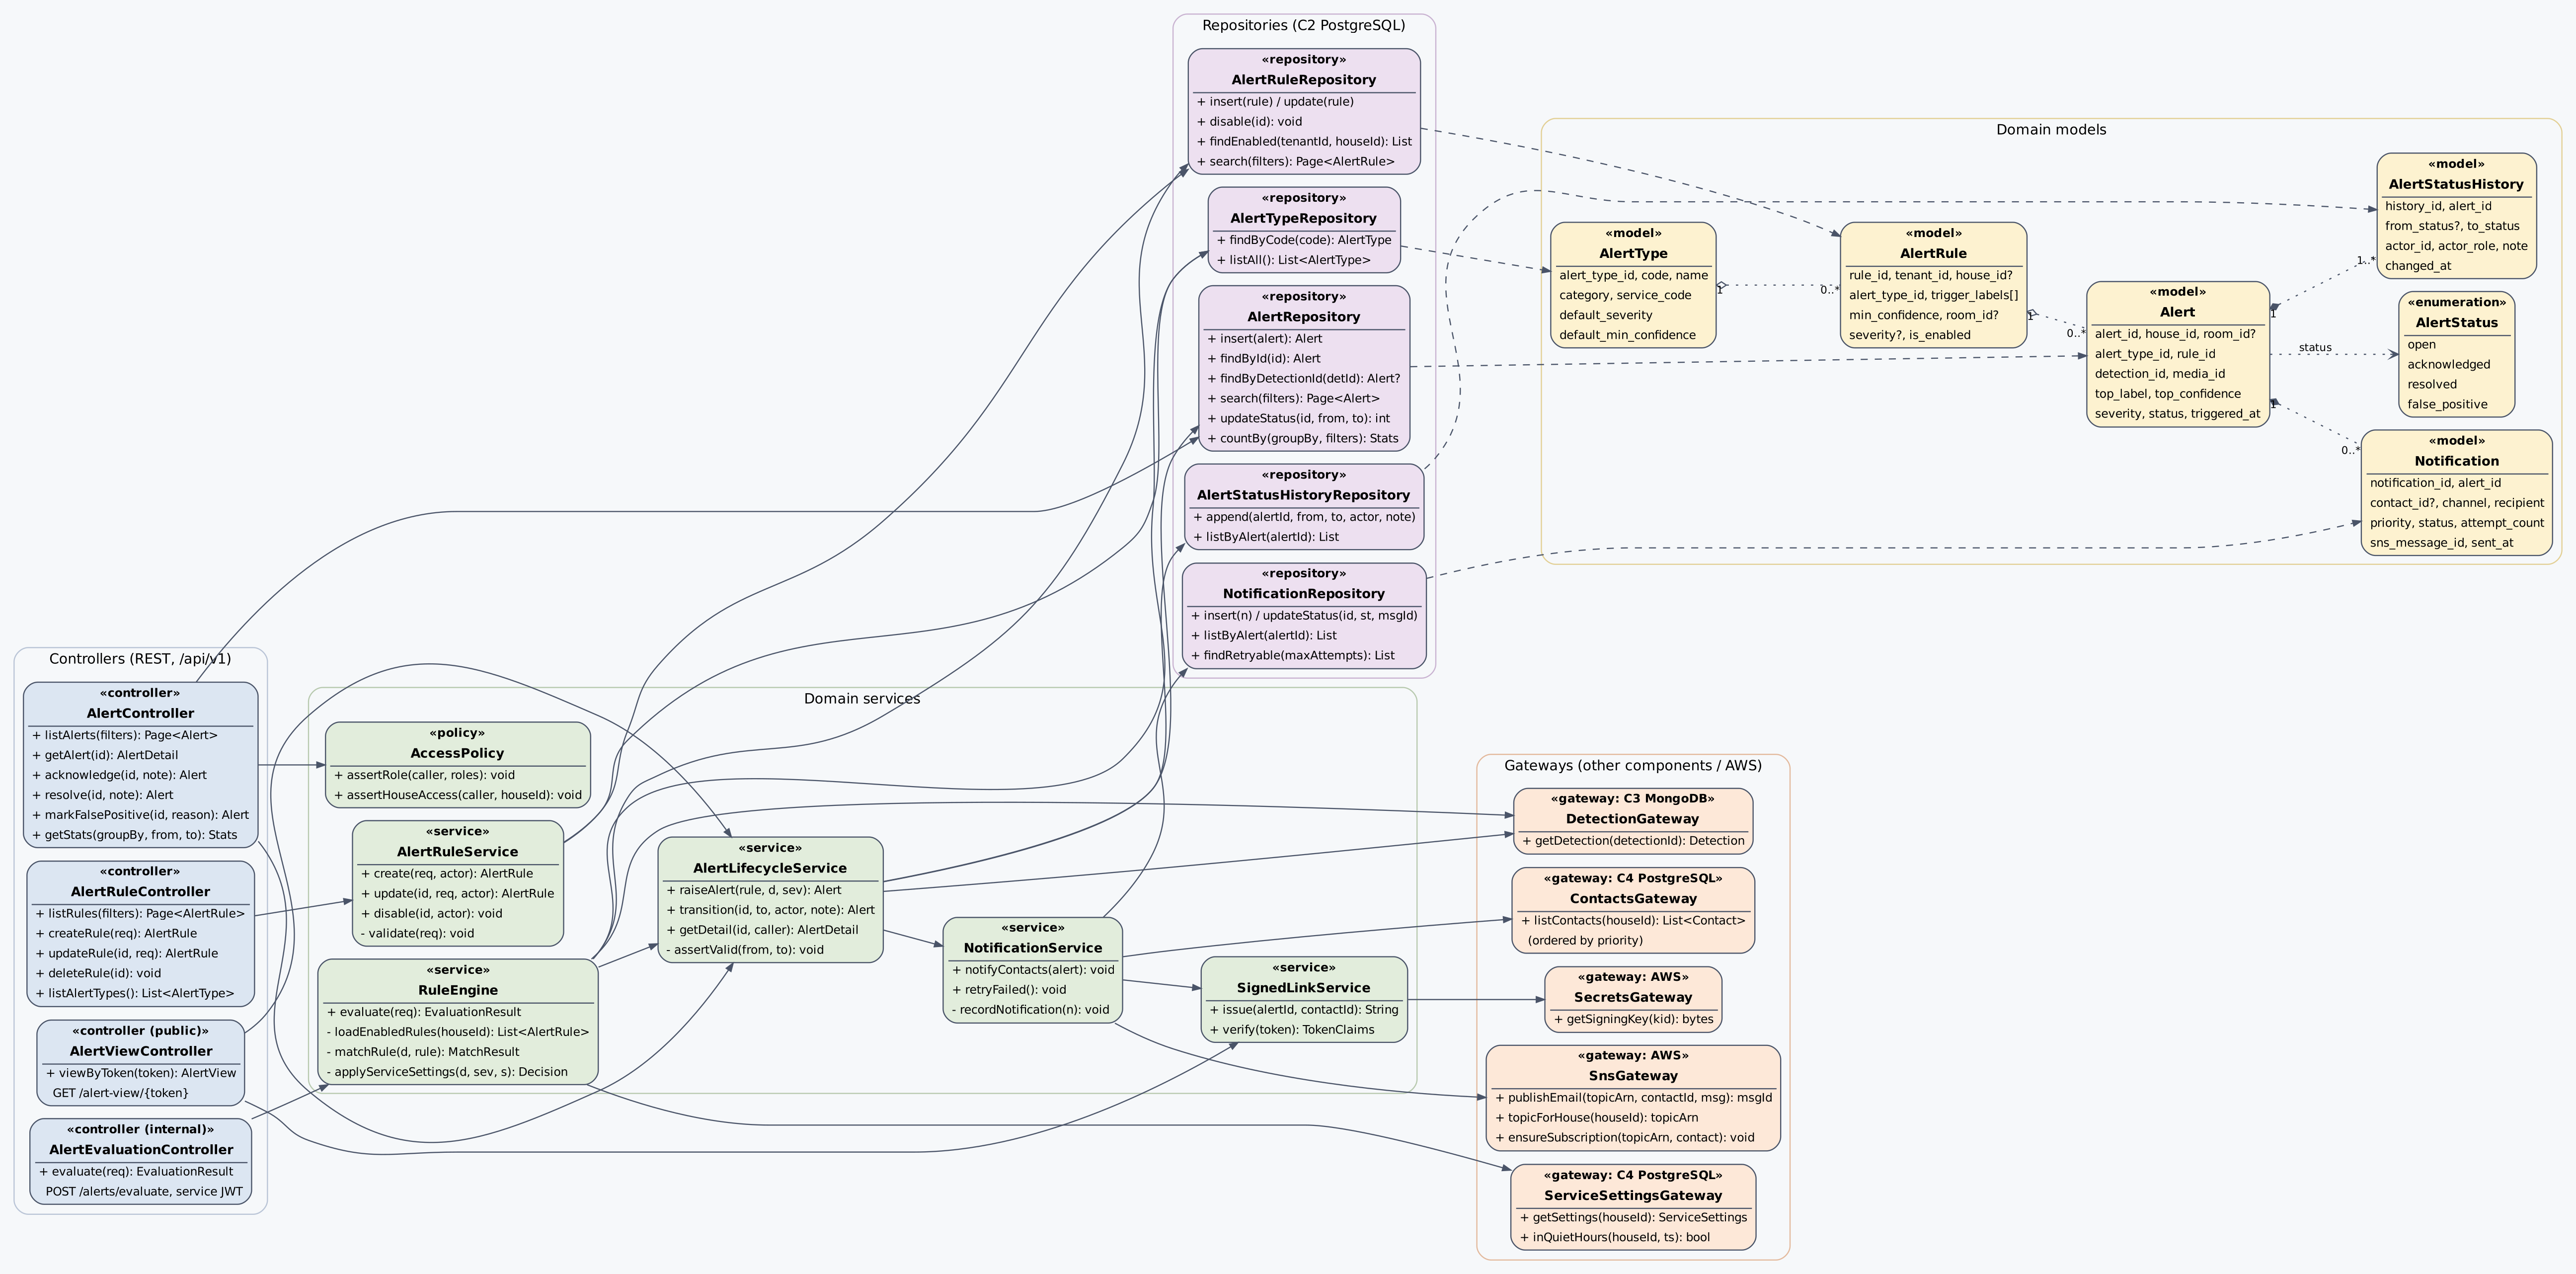
\includegraphics[width=\linewidth,height=0.86\textheight,keepaspectratio]{figures/C2/c2-class}
\captionof{figure}{C2 internal class diagram: controllers, domain services, repositories, gateways and domain models (dashed arrow = manages model; diamond = aggregation / composition)}\label{fig:c2-class}
\end{landscape}

\begin{longtable}{L{3.6cm}L{1.9cm}L{5.6cm}L{3.7cm}}
\caption{C2 class specification}\label{tab:c2-classspec}\\
\toprule
\textbf{Class} & \textbf{Stereotype} & \textbf{Responsibility} & \textbf{Collaborates with} \\
\midrule
\endfirsthead
\caption[]{C2 class specification (continued)}\\
\toprule
\textbf{Class} & \textbf{Stereotype} & \textbf{Responsibility} & \textbf{Collaborates with} \\
\midrule
\endhead
\texttt{AlertController} & controller & Alert list, detail, stats and the three lifecycle actions; maps exceptions to HTTP codes & \texttt{AccessPolicy}, \texttt{AlertLifecycle\allowbreak Service}, \texttt{AlertRepository} \\
\texttt{AlertEvaluation\allowbreak Controller} & controller & Internal evaluate endpoint; service JWT check; idempotency short-circuit & \texttt{RuleEngine}, \texttt{AlertRepository} \\
\texttt{AlertRuleController} & controller & Rule CRUD and alert-type list & \texttt{AlertRuleService}, \texttt{AccessPolicy} \\
\texttt{AlertViewController} & controller & Public signed view & \texttt{SignedLinkService}, \texttt{AlertLifecycle\allowbreak Service} \\
\texttt{RuleEngine} & service & Load rules in precedence order, apply service settings and quiet hours, choose \texttt{alert} or \texttt{no\_alert(reason)} & \texttt{AlertRuleRepository}, \texttt{AlertTypeRepository}, \texttt{DetectionGateway}, \texttt{ServiceSettings\allowbreak Gateway}, \texttt{AlertLifecycle\allowbreak Service} \\
\texttt{AlertLifecycle\allowbreak Service} & service & Create alerts; guarded transitions; history; assemble alert detail & \texttt{AlertRepository}, \texttt{AlertStatusHistory\allowbreak Repository}, \texttt{Notification\allowbreak Service}, \texttt{DetectionGateway} \\
\texttt{Notification\allowbreak Service} & service & Choose channels by severity; email contacts in priority order; retry & \texttt{ContactsGateway}, \texttt{SignedLinkService}, \texttt{SnsGateway}, \texttt{Notification\allowbreak Repository} \\
\texttt{AlertRuleService} & service & Validate and persist rules; duplicate check & \texttt{AlertRuleRepository}, \texttt{AlertTypeRepository} \\
\texttt{SignedLinkService} & service & Issue and verify HMAC tokens & \texttt{SecretsGateway} \\
\texttt{AccessPolicy} & policy & Role and house-scope checks (Table~\ref{tab:c2-access}) & JWT claims \\
\texttt{*Repository} (5) & repository & SQL access to one C2 table each; transactions per use case & PostgreSQL \\
\texttt{DetectionGateway}, \texttt{ServiceSettings\allowbreak Gateway}, \texttt{ContactsGateway} & gateway & Read-only access to C3 / C4 data & MongoDB, PostgreSQL (C4) \\
\texttt{SnsGateway}, \texttt{SecretsGateway} & gateway & AWS SDK wrappers & Amazon SNS, Secrets Manager \\
\bottomrule
\end{longtable}

\subsection{Data and database design}
C2 owns five relational tables in PostgreSQL (Figure~\ref{fig:c2-er}). Value sets use the exact enumerations
from the platform schema and are enforced with \texttt{CHECK} constraints. References to C3 and C4 records are
\emph{logical} (stored IDs, no foreign key), because those records live in other components' stores.

\figH{C2/c2-er}{0.92}{C2 entity-relationship diagram: five C2 tables (white) and the C3/C4 records they reference (grey, read-only)}{fig:c2-er}

\begin{longtable}{L{4.6cm}L{3.0cm}L{7.0cm}}
\caption{C2 data dictionary (key columns)}\label{tab:c2-dd}\\
\toprule
\textbf{Table.column} & \textbf{Type} & \textbf{Constraint / description} \\
\midrule
\endfirsthead
\caption[]{C2 data dictionary (key columns) (continued)}\\
\toprule
\textbf{Table.column} & \textbf{Type} & \textbf{Constraint / description} \\
\midrule
\endhead
\texttt{alert\_types.code}, \texttt{service\_code} & VARCHAR(40) & UNIQUE code; C4 service that must be enabled (Table~\ref{tab:c2-defaults}) \\
\texttt{alert\_types.category} & VARCHAR CHECK & \texttt{emergency}, \texttt{safety}, \texttt{security}, \texttt{wellness}, \texttt{system} \\
\texttt{alert\_rules.house\_id} & UUID NULL & NULL = all houses of the tenant \\
\texttt{alert\_rules.trigger\_labels} & TEXT[] & $\ge$ 1 label from the C3 label map \\
\texttt{alert\_rules.min\_confidence} & NUMERIC(3,2) & CHECK 0--1 \\
\texttt{alert\_rules.version}, \texttt{deleted\_at} & INT, TIMESTAMPTZ & Optimistic lock; soft delete \\
\texttt{alerts.detection\_id} & UUID & UNIQUE; logical ref to C3 \texttt{ai\_detections.\_id} (idempotency key) \\
\texttt{alerts.media\_id} & UUID & Logical ref to the C1 clip \\
\texttt{alerts.severity} & VARCHAR CHECK & \texttt{critical}, \texttt{high}, \texttt{medium}, \texttt{low} \\
\texttt{alerts.status} & VARCHAR CHECK & \texttt{open}, \texttt{acknowledged}, \texttt{resolved}, \texttt{false\_positive} \\
\texttt{alerts.triggered\_at}, \texttt{acknowledged\_at}, \texttt{resolved\_at} & TIMESTAMPTZ & Set on creation and transitions \\
\texttt{alert\_status\_history} & BIGINT identity PK & Append-only: \texttt{from\_status} (NULL on create), \texttt{to\_status}, \texttt{actor\_id}, \texttt{actor\_role}, \texttt{note}, \texttt{changed\_at} \\
\texttt{notifications.channel} & VARCHAR CHECK & \texttt{in\_app}, \texttt{email} \\
\texttt{notifications.status}, \texttt{attempt\_count} & VARCHAR CHECK, SMALLINT & \texttt{queued}, \texttt{sent}, \texttt{failed}; 0--3 \\
\texttt{notifications.contact\_id}, \texttt{priority} & UUID NULL, SMALLINT & Logical ref to C4 contact; priority order \\
\bottomrule
\end{longtable}

\textbf{Indexes.}
\begin{itemize}
\item \texttt{alerts(house\_id, status, triggered\_at DESC)}: dashboard lists.
\item \texttt{alerts(tenant\_id, triggered\_at)}: statistics.
\item \texttt{UNIQUE alerts(detection\_id)}: evaluation idempotency.
\item \texttt{alert\_rules(tenant\_id, house\_id) WHERE is\_enabled}: rule loading during evaluation.
\item Partial unique index on \texttt{alert\_rules(tenant\_id, house\_id, alert\_type\_id, room\_id) WHERE is\_enabled} (NULLs coalesced): blocks duplicate enabled rules.
\item \texttt{alert\_status\_history(alert\_id, changed\_at)}: timeline.
\item \texttt{notifications(status, created\_at) WHERE status = 'failed'}: retry job.
\end{itemize}
Retention: alerts and history are kept for 2 years; notifications for 1 year.


\subsection{Program function descriptions}
Table~\ref{tab:c2-fn} lists the key internal functions. Figure~\ref{fig:c2-eval} is the rule-evaluation
flowchart, and the pseudocode below gives evaluation, the guarded transition, notification, and the signed link.

\begin{longtable}{L{4.0cm}L{4.0cm}L{6.6cm}}
\caption{C2 key internal functions}\label{tab:c2-fn}\\
\toprule
\textbf{Function} & \textbf{Inputs $\rightarrow$ outputs} & \textbf{Logic} \\
\midrule
\endfirsthead
\caption[]{C2 key internal functions (continued)}\\
\toprule
\textbf{Function} & \textbf{Inputs $\rightarrow$ outputs} & \textbf{Logic} \\
\midrule
\endhead
\texttt{RuleEngine.\allowbreak evaluate(req)} & detection snapshot $\rightarrow$ \texttt{EvaluationResult} & Idempotency check; verify detection; walk rules in precedence order; first full match raises an alert, else return the most specific \texttt{no\_alert} reason \\
\texttt{RuleEngine.\allowbreak loadEnabledRules(t, h)} & tenant, house $\rightarrow$ rule list & House rules first, then tenant rules for alert types the house has no rule for; each group ordered by severity rank \\
\texttt{AlertLifecycleService.\allowbreak raiseAlert} & rule, detection, severity $\rightarrow$ Alert & One transaction: insert alert + history; after commit call \texttt{notifyContacts} \\
\texttt{AlertLifecycleService.\allowbreak transition} & alert id, target, actor, note $\rightarrow$ Alert & \texttt{assertValid}; conditional update on the current status; append history; 409 on invalid or lost update \\
\texttt{NotificationService.\allowbreak notifyContacts} & alert $\rightarrow$ void & Always an \texttt{in\_app} record; for critical/high, email each contact in priority order with its own signed link \\
\texttt{NotificationService.\allowbreak retryFailed} & none $\rightarrow$ void & Every 60 s: re-publish \texttt{failed} emails with \texttt{attempt\_count} $<$ 3 whose backoff (1, 2, 4 min) has passed \\
\texttt{SignedLinkService.\allowbreak issue / verify} & alert, contact $\leftrightarrow$ token & HMAC-SHA256 over \texttt{\{aid, cid, exp, kid\}}; constant-time compare; check \texttt{exp} \\
\texttt{AccessPolicy.\allowbreak assertHouseAccess} & caller, house $\rightarrow$ void & Owner: house in \texttt{house\_ids} claim. Staff: house in the caller's tenant. Else 403 \\
\bottomrule
\end{longtable}

\figH{C2/c2-eval-flow}{0.46}{Rule evaluation flowchart: validate, idempotency check, verify detection, walk rules in precedence order, apply quiet hours, raise or return no\_alert with reason}{fig:c2-eval}

\begin{Shaded}
\begin{Code}
function evaluate(req):                                   # POST /alerts/evaluate
    existing = alerts.findByDetectionId(req.detection_id)
    if existing: return Result(decision="alert", alert_id=existing.id, duplicate=True)
    d = detections.getDetection(req.detection_id)          # C3 gateway, authoritative copy
    if d is None or d.house_id != req.house_id: raise http(422, "validation_error")
    settings = serviceSettings.get(d.house_id)               # from C4 (also gives tenant_id)
    rules    = loadEnabledRules(settings.tenant_id, d.house_id)  # house rules first, then tenant defaults
    best_miss = "no_rule_match"                              # most specific reason seen so far
    for rule in rules:
        if rule.alert_type.service_code not in settings.enabled:
            best_miss = moreSpecific(best_miss, "service_disabled"); continue
        if d.top_label not in rule.trigger_labels: continue
        threshold = clamp(rule.min_confidence + SENS[settings.sensitivity], 0.05, 0.95)  # low +0.10, high -0.10
        if d.top_confidence < threshold:
            best_miss = moreSpecific(best_miss, "below_threshold"); continue
        if rule.room_id is not None and rule.room_id != d.room_id:
            best_miss = moreSpecific(best_miss, "room_mismatch"); continue
        sev = rule.severity or rule.alert_type.default_severity
        if settings.inQuietHours(now(), house_tz) and sev in ("medium", "low"):  # critical/high bypass
            return logDecision(d, "no_alert", "quiet_hours")
        alert = lifecycle.raiseAlert(rule, d, sev)            # insert + history, then notify
        return logDecision(d, "alert", alert.id)
    return logDecision(d, "no_alert", best_miss)
# precedence of reasons: room_mismatch > below_threshold > service_disabled > no_rule_match

function transition(alertId, toStatus, actor, note):
    allowed = { "open": ["acknowledged","false_positive"],
                "acknowledged": ["resolved","false_positive"] }  # resolved, false_positive: terminal
    alert = alerts.findById(alertId) or raise http(404, "not_found")
    accessPolicy.assertHouseAccess(actor, alert.house_id)
    if toStatus == "false_positive" and not note: raise http(422, "validation_error", "reason")
    if toStatus not in allowed.get(alert.status, []):
        raise http(409, "invalid_state", {"from": alert.status, "to": toStatus})
    begin transaction
        rows = alerts.updateStatus(alertId, from=alert.status, to=toStatus)  # WHERE status = from
        if rows == 0: rollback; raise http(409, "invalid_state", "changed concurrently")
        history.append(alertId, alert.status, toStatus, actor.id, actor.role, note)
    commit
    return alerts.findById(alertId)

function notifyContacts(alert):
    notifications.insert(alert.id, channel="in_app", status="sent")
    if alert.severity not in ("critical", "high"): return
    topic = sns.topicForHouse(alert.house_id)
    for c in contacts.listContacts(alert.house_id) ordered by c.priority:   # 1 = first
        sns.ensureSubscription(topic, c)                     # email protocol + filter {contact_id}
        n = notifications.insert(alert.id, c.id, "email", c.email, c.priority, status="queued")
        link = BASE_URL + "/alert-view/" + signedLinks.issue(alert.id, c.id)  # exp = triggered_at+24h
        try:
            msgId = sns.publishEmail(topic, c.id, renderEmail(alert, link))
            notifications.updateStatus(n.id, "sent", msgId)
        except SnsError as e:
            notifications.markFailed(n.id, attempt=1, error=str(e))   # picked up by retryFailed()
\end{Code}
\end{Shaded}

\subsection{Behavior: alert state machine}
Figure~\ref{fig:c2-state} is the alert status machine. The only transitions are \texttt{open} to
\texttt{acknowledged}, \texttt{acknowledged} to \texttt{resolved}, and \texttt{open} or
\texttt{acknowledged} to \texttt{false\_positive}. The states \texttt{resolved} and
\texttt{false\_positive} are terminal. Any other requested change returns \texttt{409 invalid\_state}.
Table~\ref{tab:c2-dt-trans} in Section~\ref{sec:c2-bl} gives every event against every state. Each transition is guarded by the caller's house access (\texttt{AccessPolicy}) and appends a history row with actor, role, time and note.

\figH{C2/c2-alert-state}{0.95}{Alert status machine: open, acknowledged, resolved, false\_positive, with 409 on any invalid transition}{fig:c2-state}



\textbf{Notification sub-state and retry.} Each \texttt{notifications} row moves \texttt{queued} $\rightarrow$
\texttt{sent} on a successful SNS publish, or \texttt{queued} $\rightarrow$ \texttt{failed}. A \texttt{failed}
row with \texttt{attempt\_count} $<$ 3 goes back to \texttt{sent} or stays \texttt{failed} on each retry. At three
attempts it stays \texttt{failed} for good, which is shown in Alert Detail and counted in a CloudWatch metric.
The alert's own status does not depend on notification status.

\subsection{Behavior: sequence diagrams}
Two sequence diagrams cover the two main C2 use cases.

\textbf{(a) Evaluate rules and raise an alert (UC-04)}, Figure~\ref{fig:c2-seq}. The C3 worker calls
\texttt{/alerts/evaluate}. The controller first checks for an existing alert for the detection (a retry). Otherwise
the rule engine reads the detection and the house's settings, the alert is inserted \texttt{open}, history is appended,
and the notifier emails each contact in priority order with that contact's signed link.

\figH{C2/c2-seq-evaluate}{1.0}{Sequence (a): C3 triggers evaluation, an alert is raised and contacts are emailed in priority order through SNS}{fig:c2-seq}

\textbf{(b) Owner handles the alert}, Figure~\ref{fig:c2-seq-handle}. The \emph{house owner}, through the C4
dashboard, opens Alert Detail, then acknowledges and resolves. Each transition is guarded by the state machine and
by a conditional update that detects concurrent changes.

\figH{C2/c2-seq-handle}{0.82}{Sequence (b): house owner views, acknowledges and resolves an alert; invalid or concurrent transitions return 409}{fig:c2-seq-handle}

The signed alert view and rule creation follow the decision tables in Section~\ref{sec:c2-bl}
(Tables~\ref{tab:c2-dt-rule} and \ref{tab:c2-dt-link}).

% ============================================================================
\section{Component Business Logic}\label{sec:c2-bl}

\subsection{Rule-match decision table}
For each rule in precedence order, the first rule whose conditions all hold raises the alert. If no rule
matches, the most specific reason seen is returned. ``Adj.\ min'' is the rule's minimum confidence shifted by the
house sensitivity stored in C4 (low $+0.10$, medium $0$, high $-0.10$, clamped to 0.05--0.95). Quiet hours are read in
the house's own time zone (C1 \texttt{houses.timezone}); only medium and low alerts are held.

\begin{longtable}{L{1.9cm}L{2.0cm}L{1.6cm}L{1.6cm}L{2.2cm}L{2.6cm}L{2.3cm}}
\caption{Rule-match decision table}\label{tab:c2-dt-match}\\
\toprule
\textbf{Service on} & \textbf{Label in rule} & \textbf{Conf $\geq$ adj. min} & \textbf{Room} & \textbf{Quiet hrs} & \textbf{Action} & \textbf{Reason} \\
\midrule
\endfirsthead
\caption[]{Rule-match decision table (continued)}\\
\toprule
\textbf{Service on} & \textbf{Label in rule} & \textbf{Conf $\geq$ adj. min} & \textbf{Room} & \textbf{Quiet hrs} & \textbf{Action} & \textbf{Reason} \\
\midrule
\endhead
no & -- & -- & -- & -- & No alert & \texttt{service\_disabled} \\
yes & no & -- & -- & -- & No alert & \texttt{no\_rule\_match} \\
yes & yes & no & -- & -- & No alert & \texttt{below\_threshold} \\
yes & yes & yes & mismatch & -- & No alert & \texttt{room\_mismatch} \\
yes & yes & yes & match & yes, medium/low & Suppressed & \texttt{quiet\_hours} \\
yes & yes & yes & match & yes, critical/high & Raise alert (bypass quiet hours) & -- \\
yes & yes & yes & match & no & Raise alert & -- \\
\bottomrule
\end{longtable}

\textbf{Rule precedence.} A house rule overrides the tenant default for the same alert type; among matching
rules of different types the highest severity wins, then a room-specific rule before an any-room rule, then the oldest
rule. A detection that already has an alert never creates another.

\subsection{Default minimum confidence per alert type (TBD-2, resolved)}
This resolves the item the SRS parked as TBD-2. Each alert type carries a default minimum confidence,
aligned with the home labels and thresholds in the C3 label map. These defaults will be validated in D3; a
per-house rule may override them.

\begin{longtable}{L{2.6cm}L{2.6cm}L{2.0cm}L{2.0cm}L{1.6cm}L{2.6cm}}
\caption{Alert type defaults}\label{tab:c2-defaults}\\
\toprule
\textbf{Alert type} & \textbf{Trigger label (C3)} & \textbf{Category} & \textbf{Default sev.} & \textbf{Min conf.} & \textbf{C4 service code} \\
\midrule
\endfirsthead
\caption[]{Alert type defaults (continued)}\\
\toprule
\textbf{Alert type} & \textbf{Trigger label (C3)} & \textbf{Category} & \textbf{Default sev.} & \textbf{Min conf.} & \textbf{C4 service code} \\
\midrule
\endhead
\texttt{smoke} & \texttt{smoke\_alarm} & emergency & critical & 0.50 & \texttt{fire\_safety} \\
\texttt{distress} & \texttt{distress\_sound} & emergency & critical & 0.60 & \texttt{distress} \\
\texttt{intrusion} & \texttt{glass\_break} & security & high & 0.55 & \texttt{intrusion} \\
\texttt{fall} & \texttt{fall\_indicator} & safety & high & 0.65 & \texttt{fall} \\
\texttt{wellness\_cough} & \texttt{cough} & wellness & low & 0.55 & \texttt{wellness} \\
\texttt{presence} & \texttt{speech} & wellness & low & 0.50 & \texttt{presence} \\
\texttt{pet} & \texttt{dog} & wellness & low & 0.55 & \texttt{pet} \\
\bottomrule
\end{longtable}

\subsection{Notification channel by severity}
\begin{longtable}{L{3.0cm}L{5.0cm}L{6.0cm}}
\caption{Notification channels}\\
\toprule
\textbf{Severity} & \textbf{Channels} & \textbf{Recipients} \\
\midrule
\endfirsthead
\caption[]{Notification channels (continued)}\\
\toprule
\textbf{Severity} & \textbf{Channels} & \textbf{Recipients} \\
\midrule
\endhead
\texttt{critical}, \texttt{high} & \texttt{email} + \texttt{in\_app} & Emergency contacts (email, one signed link each, priority order) and signed-in users \\
\texttt{medium}, \texttt{low} & \texttt{in\_app} & Signed-in users of the house only \\
\bottomrule
\end{longtable}

\subsection{Alert transition decision table}
\begin{longtable}{L{3.2cm}L{3.4cm}L{3.4cm}L{4.6cm}}
\caption{Alert transition decision table}\label{tab:c2-dt-trans}\\
\toprule
\textbf{Current status} & \textbf{acknowledge} & \textbf{resolve} & \textbf{false positive (with reason)} \\
\midrule
\endfirsthead
\caption[]{Alert transition decision table (continued)}\\
\toprule
\textbf{Current status} & \textbf{acknowledge} & \textbf{resolve} & \textbf{false positive (with reason)} \\
\midrule
\endhead
\texttt{open} & $\rightarrow$ acknowledged & 409 & $\rightarrow$ false\_positive \\
\texttt{acknowledged} & 409 & $\rightarrow$ resolved & $\rightarrow$ false\_positive \\
\texttt{resolved} & 409 & 409 & 409 \\
\texttt{false\_positive} & 409 & 409 & 409 \\
\bottomrule
\end{longtable}

\subsection{Access control decision table}
\begin{longtable}{L{4.6cm}L{2.5cm}L{2.5cm}L{2.4cm}L{2.6cm}}
\caption{Who may call what}\label{tab:c2-access}\\
\toprule
\textbf{Operation} & \textbf{house\_owner} & \textbf{cloud\_staff} & \textbf{C3 service} & \textbf{Token holder} \\
\midrule
\endfirsthead
\caption[]{Who may call what (continued)}\\
\toprule
\textbf{Operation} & \textbf{house\_owner} & \textbf{cloud\_staff} & \textbf{C3 service} & \textbf{Token holder} \\
\midrule
\endhead
List / view / stats of alerts & own houses & tenant & no & no \\
Acknowledge, resolve, false positive & own houses & tenant & no & no \\
List alert types & yes & yes & no & no \\
Create / edit / disable rules & no (403) & tenant & no & no \\
Evaluate detection & no & no & yes & no \\
Signed alert view & -- & -- & -- & one alert, 24 h \\
\bottomrule
\end{longtable}

\subsection{Rule validation decision table}
\begin{longtable}{L{1.8cm}L{2.2cm}L{2.0cm}L{2.0cm}L{2.0cm}L{4.4cm}}
\caption{POST / PUT /alert-rules validation}\label{tab:c2-dt-rule}\\
\toprule
\textbf{Type exists} & \textbf{Labels in map, $\ge 1$} & \textbf{$0\le$ conf $\le 1$} & \textbf{Room in house} & \textbf{Duplicate enabled} & \textbf{Result} \\
\midrule
\endfirsthead
\caption[]{POST / PUT /alert-rules validation (continued)}\\
\toprule
\textbf{Type exists} & \textbf{Labels in map, $\ge 1$} & \textbf{$0\le$ conf $\le 1$} & \textbf{Room in house} & \textbf{Duplicate enabled} & \textbf{Result} \\
\midrule
\endhead
no & -- & -- & -- & -- & 422 \texttt{alert\_type\_code} \\
yes & no & -- & -- & -- & 422 \texttt{trigger\_labels} \\
yes & yes & no & -- & -- & 422 \texttt{min\_confidence} \\
yes & yes & yes & no & -- & 422 \texttt{room\_id} \\
yes & yes & yes & yes / any & yes & 409 \texttt{duplicate\_rule} \\
yes & yes & yes & yes / any & no & 201 Created (200 on PUT) \\
\bottomrule
\end{longtable}

\subsection{Signed link decision table}
\begin{longtable}{L{3.0cm}L{3.0cm}L{2.6cm}L{2.6cm}L{3.4cm}}
\caption{GET /alert-view/\{token\} outcome}\label{tab:c2-dt-link}\\
\toprule
\textbf{Well-formed} & \textbf{Signature valid} & \textbf{Not expired} & \textbf{Alert exists} & \textbf{Response} \\
\midrule
\endfirsthead
\caption[]{GET /alert-view/\{token\} outcome (continued)}\\
\toprule
\textbf{Well-formed} & \textbf{Signature valid} & \textbf{Not expired} & \textbf{Alert exists} & \textbf{Response} \\
\midrule
\endhead
no & -- & -- & -- & 404 \\
yes & no & -- & -- & 404 \\
yes & yes & no & -- & 401 \texttt{token\_expired} \\
yes & yes & yes & no & 404 \\
yes & yes & yes & yes & 200 read-only view \\
\bottomrule
\end{longtable}

% ============================================================================
\section{Component Graphic User Interface Design}

\subsection{GUI style}
C2's surfaces live in the owner and cloud workspaces of the React single-page application served by C4,
plus one stand-alone public page. Severity is shown with an icon and a word, never colour alone, so the
alert list is readable without colour vision. The external signed alert view is a minimal, read-only page
with no navigation. Table~\ref{tab:c2-style} fixes the style rules.

\begin{longtable}{L{3.0cm}L{11.8cm}}
\caption{C2 GUI style guide}\label{tab:c2-style}\\
\toprule
\textbf{Element} & \textbf{Rule} \\
\midrule
\endfirsthead
\caption[]{C2 GUI style guide (continued)}\\
\toprule
\textbf{Element} & \textbf{Rule} \\
\midrule
\endhead
Layout & Shared top navigation and breadcrumb; content in a 12-column grid; cards with 6 px radius. Alert Detail is a 2-column grid that becomes one column under 768 px. \\
Severity encoding & critical: red, triangle; high: amber, diamond; medium: blue, square; low: grey, circle. The word is always printed next to the icon. \\
Status chip & \texttt{open} (filled dot), \texttt{acknowledged}, \texttt{resolved}, \texttt{false\_positive}, each with a distinct icon and label. \\
Actions & One primary button per view (filled navy). Secondary actions are outlined. Destructive actions are outlined red and need a confirm dialog. A button the state machine does not allow is shown disabled with a tooltip, not hidden. \\
Feedback & Success toast after each action; 409 shows ``This alert was changed by someone else'' and reloads; 422 shows inline field errors. \\
Accessibility & WCAG 2.1 AA contrast; full keyboard operation; ARIA live region announces new critical alerts; clip player has captions-off notice and keyboard controls. \\
\bottomrule
\end{longtable}

\subsection{Storyboard}
Figure~\ref{fig:c2-story} is the storyboard. In path~A, a detection raises an alert (1). The owner sees it in the live
feed (2), opens Alert Detail, reviews the clip and the AI labels, and acknowledges it (3). They then resolve it or
mark it a false positive (4). In path~B, an emergency contact receives an email (5) and opens the signed alert view
to see the same alert read-only (6). Separately, cloud staff open Alert Rules (7) to tune a threshold (8).

\figH{C2/c2-storyboard}{1.0}{C2 storyboard: path A, the owner handles an alert; path B, an emergency contact views it and staff tune a rule}{fig:c2-story}

\subsection{Function partition tree}
Figure~\ref{fig:c2-gui-tree} shows the C2 GUI tree: Alert Detail, Alert Rules and the read-only
Alert View, with their function buttons.

\figH{C2/c2-gui-tree}{0.48}{C2 GUI function partition: Alert Detail, Alert Rules and the signed Alert View}{fig:c2-gui-tree}

\subsection{UI markup diagram and wireframes}
Figure~\ref{fig:c2-wireframe} is the marked-up wireframe of Alert Detail. The numbered callouts are defined in
Table~\ref{tab:c2-markup}: which template renders each element, which API feeds it, and how it behaves.

\figH{C2/c2-wireframe-alertdetail}{0.78}{UI markup of Alert Detail: evidence, AI labels, status timeline, notified contacts and lifecycle actions (Resolve disabled while open)}{fig:c2-wireframe}

\begin{longtable}{L{0.6cm}L{3.0cm}L{3.0cm}L{3.6cm}L{4.6cm}}
\caption{Alert Detail markup legend}\label{tab:c2-markup}\\
\toprule
\textbf{\#} & \textbf{Element} & \textbf{Template} & \textbf{Data source} & \textbf{Behaviour} \\
\midrule
\endfirsthead
\caption[]{Alert Detail markup legend (continued)}\\
\toprule
\textbf{\#} & \textbf{Element} & \textbf{Template} & \textbf{Data source} & \textbf{Behaviour} \\
\midrule
\endhead
1 & Top navigation & AppShell & JWT claims (role) & Owner sees Dashboard and Alerts; staff also see Alert Rules \\
2 & Severity badge & SeverityBadge & \texttt{alert.severity} & Icon + word \\
3 & Title and meta & PageHeader & \texttt{GET /alerts/\{id\}} & Type, room, house, time \\
4 & Status chip & StatusChip & \texttt{alert.status} & Updates after each action \\
5 & Evidence clip & ClipPlayer & C1 \texttt{GET /clips/\{media\_id\}/\allowbreak playback-url} & Play/pause; keyboard accessible \\
6 & AI labels & ConfidenceBars & \texttt{evidence.labels} & Matched label ticked; rule threshold shown \\
7 & Status timeline & Timeline & \texttt{timeline[]} & Actor, time and note per step \\
8 & Contacts notified & DataTable & \texttt{notifications[]} & Sent / retry n/3 / failed \\
9 & Action bar & ActionBar & \texttt{alert.status} + Table~\ref{tab:c2-dt-trans} & Buttons enabled only for allowed transitions; false positive opens a confirm dialog \\
10 & Note field & TextArea & -- & Optional for acknowledge/resolve; required for false positive \\
\bottomrule
\end{longtable}

Figure~\ref{fig:c2-wf-rules} is the Alert Rules page for cloud staff: (1) the filter bar and Add rule, (2) the
paginated rules table, (3) the create/edit panel with inline validation that follows the rule validation table.
Figure~\ref{fig:c2-wf-view} is the public signed alert view and its expired-link and invalid-link states.

\figH{C2/c2-wireframe-rules}{0.82}{Alert Rules wireframe (cloud\_staff): filter bar, rules table and edit panel}{fig:c2-wf-rules}

\figH{C2/c2-wireframe-alertview}{0.72}{Signed Alert View wireframe (public, mobile-first): valid view, expired link (401) and unrecognised link (404)}{fig:c2-wf-view}

\subsection{GUI templates}
C2 reuses the shared component library so its pages match the rest of the dashboard
(Table~\ref{tab:c2-templates}).

\begin{longtable}{L{3.0cm}L{4.0cm}L{7.8cm}}
\caption{GUI templates used by C2}\label{tab:c2-templates}\\
\toprule
\textbf{Template} & \textbf{Used on} & \textbf{Props / behaviour} \\
\midrule
\endfirsthead
\caption[]{GUI templates used by C2 (continued)}\\
\toprule
\textbf{Template} & \textbf{Used on} & \textbf{Props / behaviour} \\
\midrule
\endhead
AppShell & Alert Detail, Alert Rules & Role-aware navigation, breadcrumb, toasts \\
DataTable & Alerts list (C4), rules table, contacts & \texttt{columns}, \texttt{rows}, \texttt{page}, \texttt{onSort}, \texttt{onRowClick}; server-side pagination \\
SeverityBadge & All alert views & \texttt{severity} $\rightarrow$ icon + word + colour \\
StatusChip & All alert views & \texttt{status} $\rightarrow$ icon + label \\
ClipPlayer & Alert Detail, Alert View & \texttt{src} (pre-signed URL), \texttt{duration} \\
ConfidenceBars & Alert Detail, Alert View & \texttt{labels[]}, \texttt{threshold}, \texttt{matched} \\
Timeline & Alert Detail & \texttt{events[]} with actor, time, note \\
ActionBar & Alert Detail & \texttt{allowedActions} computed from status; confirm dialog for destructive actions \\
FormPanel & Alert Rules & Field components with inline validation messages from the 422 \texttt{details} \\
PublicCard & Alert View & Stand-alone, no navigation, mobile-first \\
\bottomrule
\end{longtable}

